% !TeX root = ../rasd.tex
\section{External Interface Requirements}

\subsection{User Interfaces}
\begin{figure}[H]
      \centering
      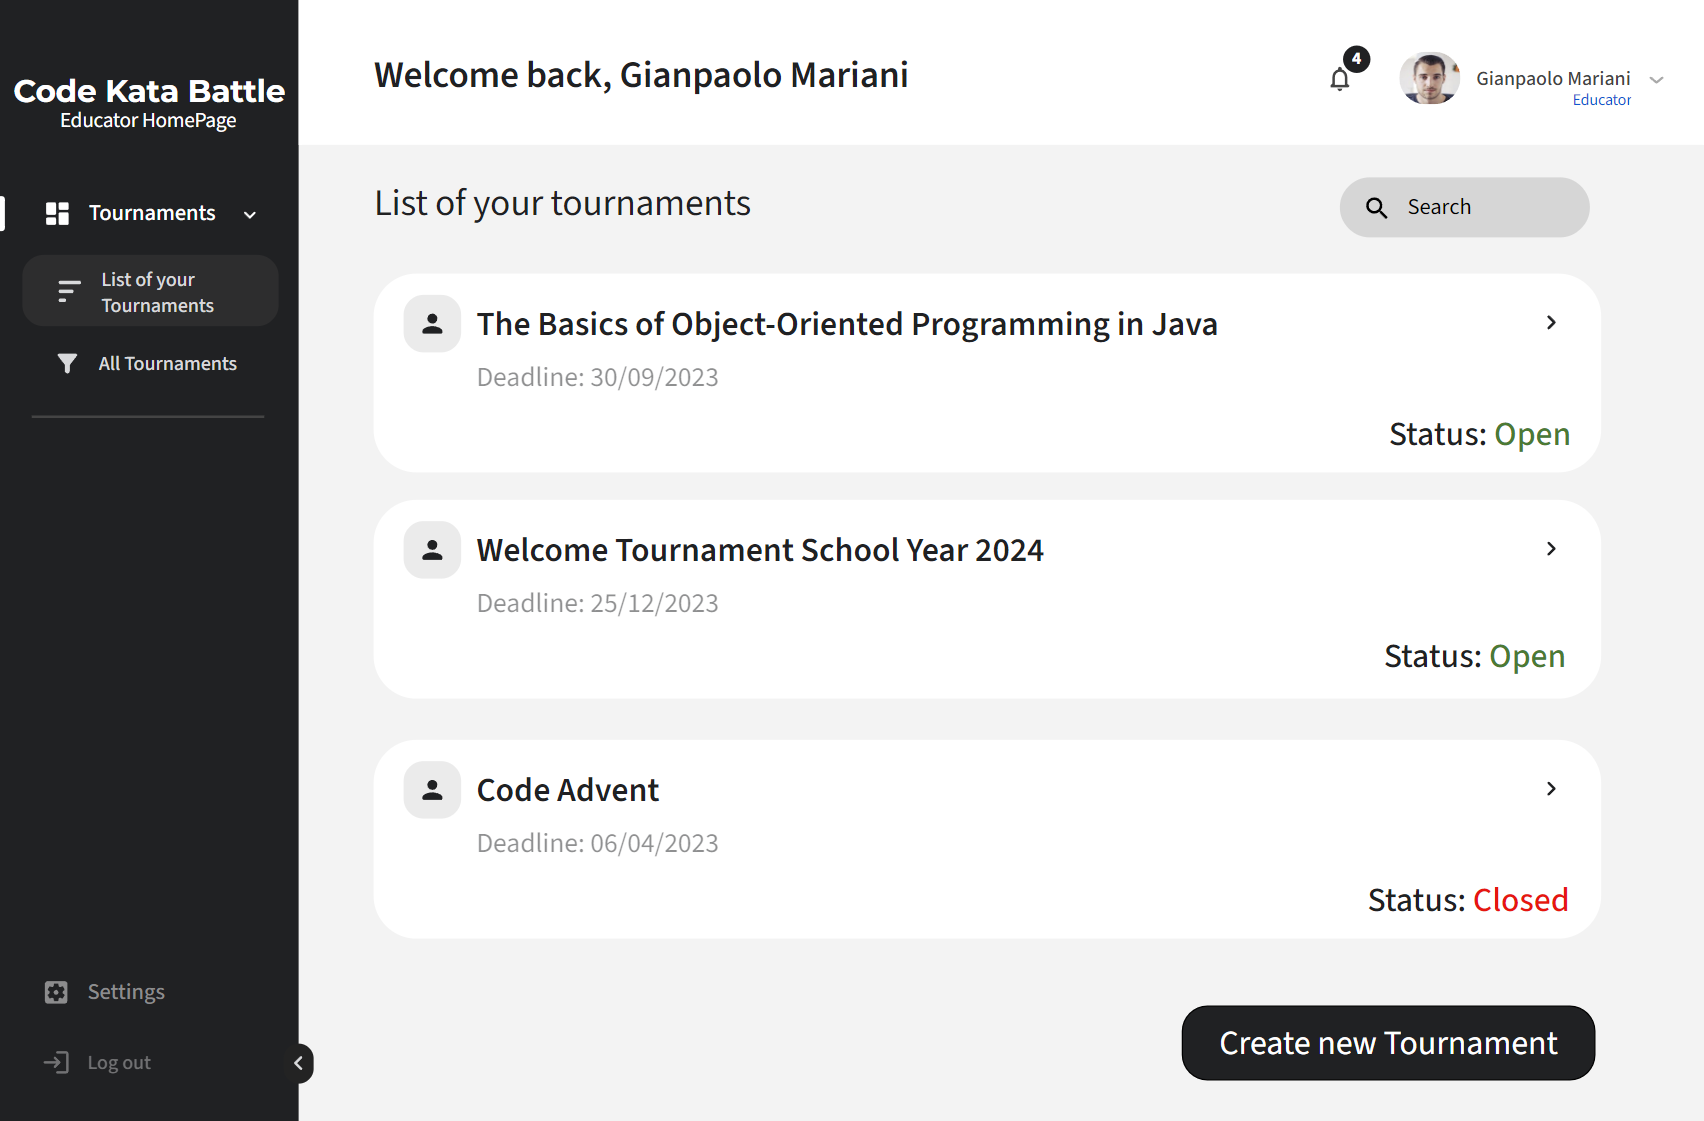
\includegraphics[width=\textwidth]{../images/homepage-educator.png}
      \caption{HomePage Educator}
      \label{fig:HomePage Educator}
\end{figure}
\begin{figure}[H]
      \centering
      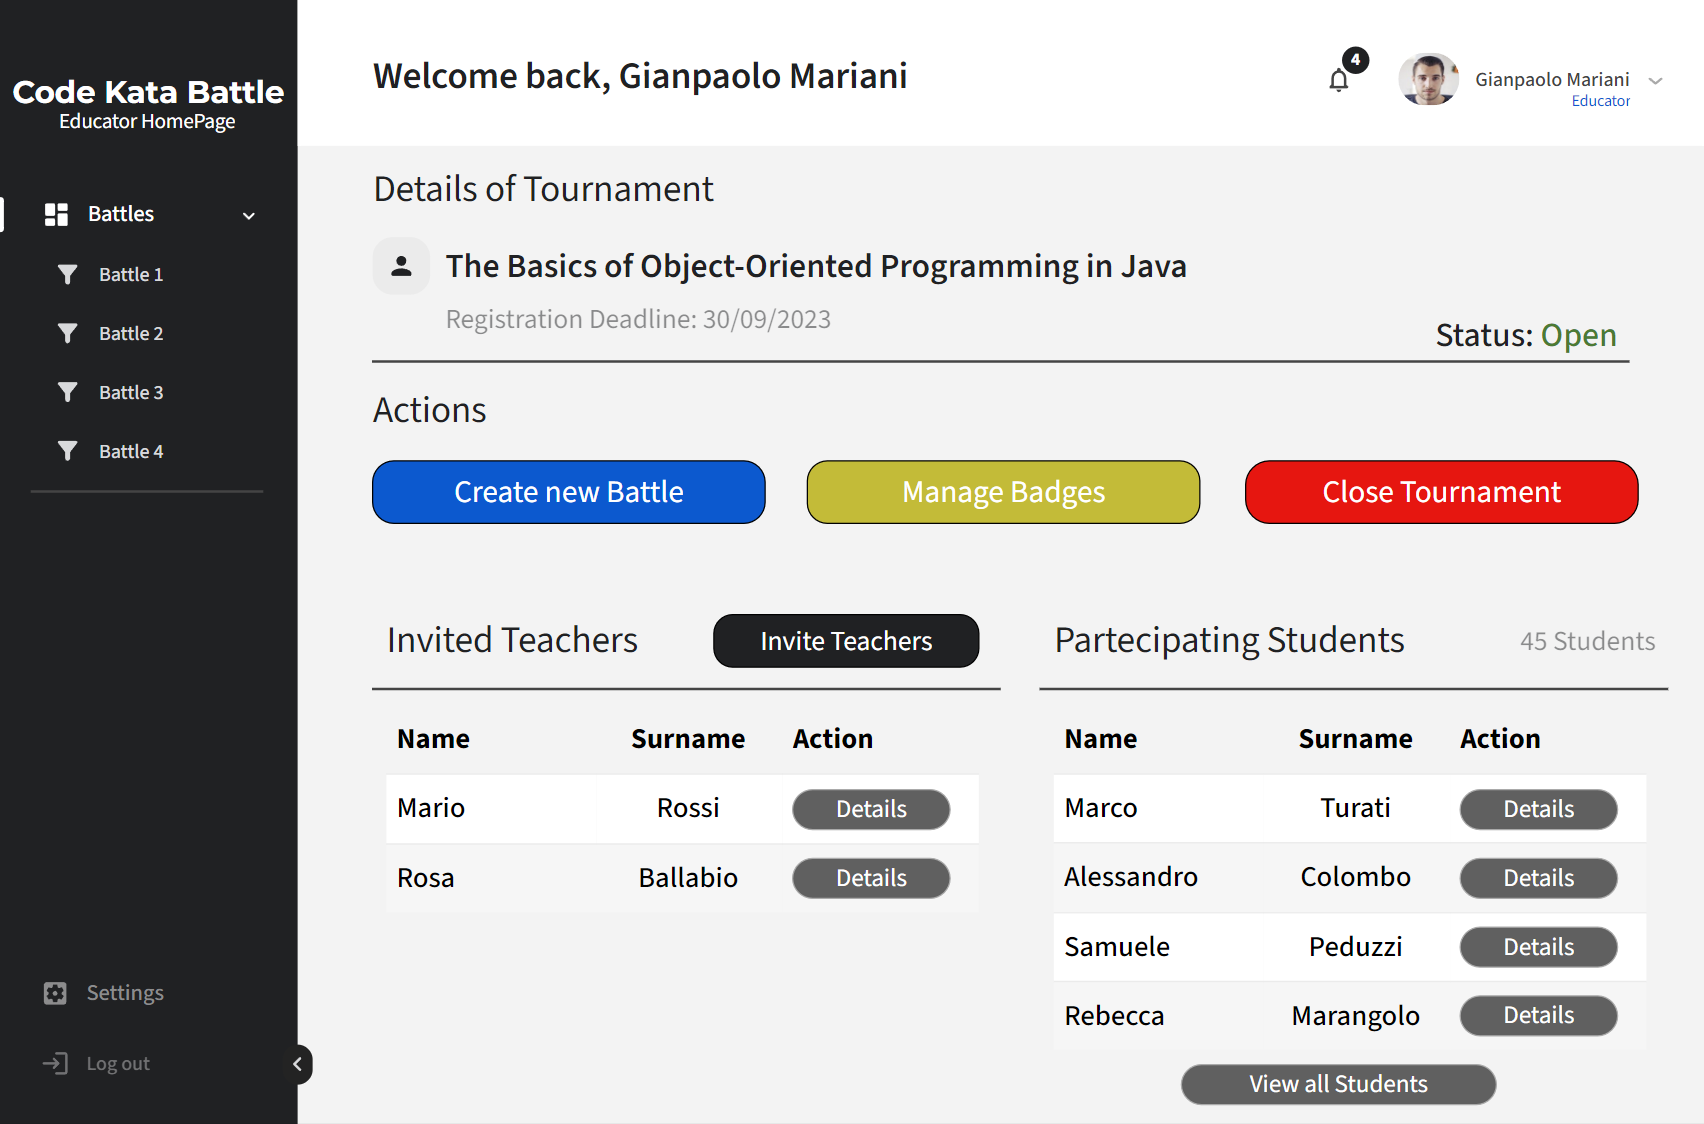
\includegraphics[width=\textwidth]{../images/details-tournament-educator.png}
      \caption{Details Tournament Educator}
      \label{fig:Details Tournament Educator}
\end{figure}
\begin{figure}[H]
      \centering
      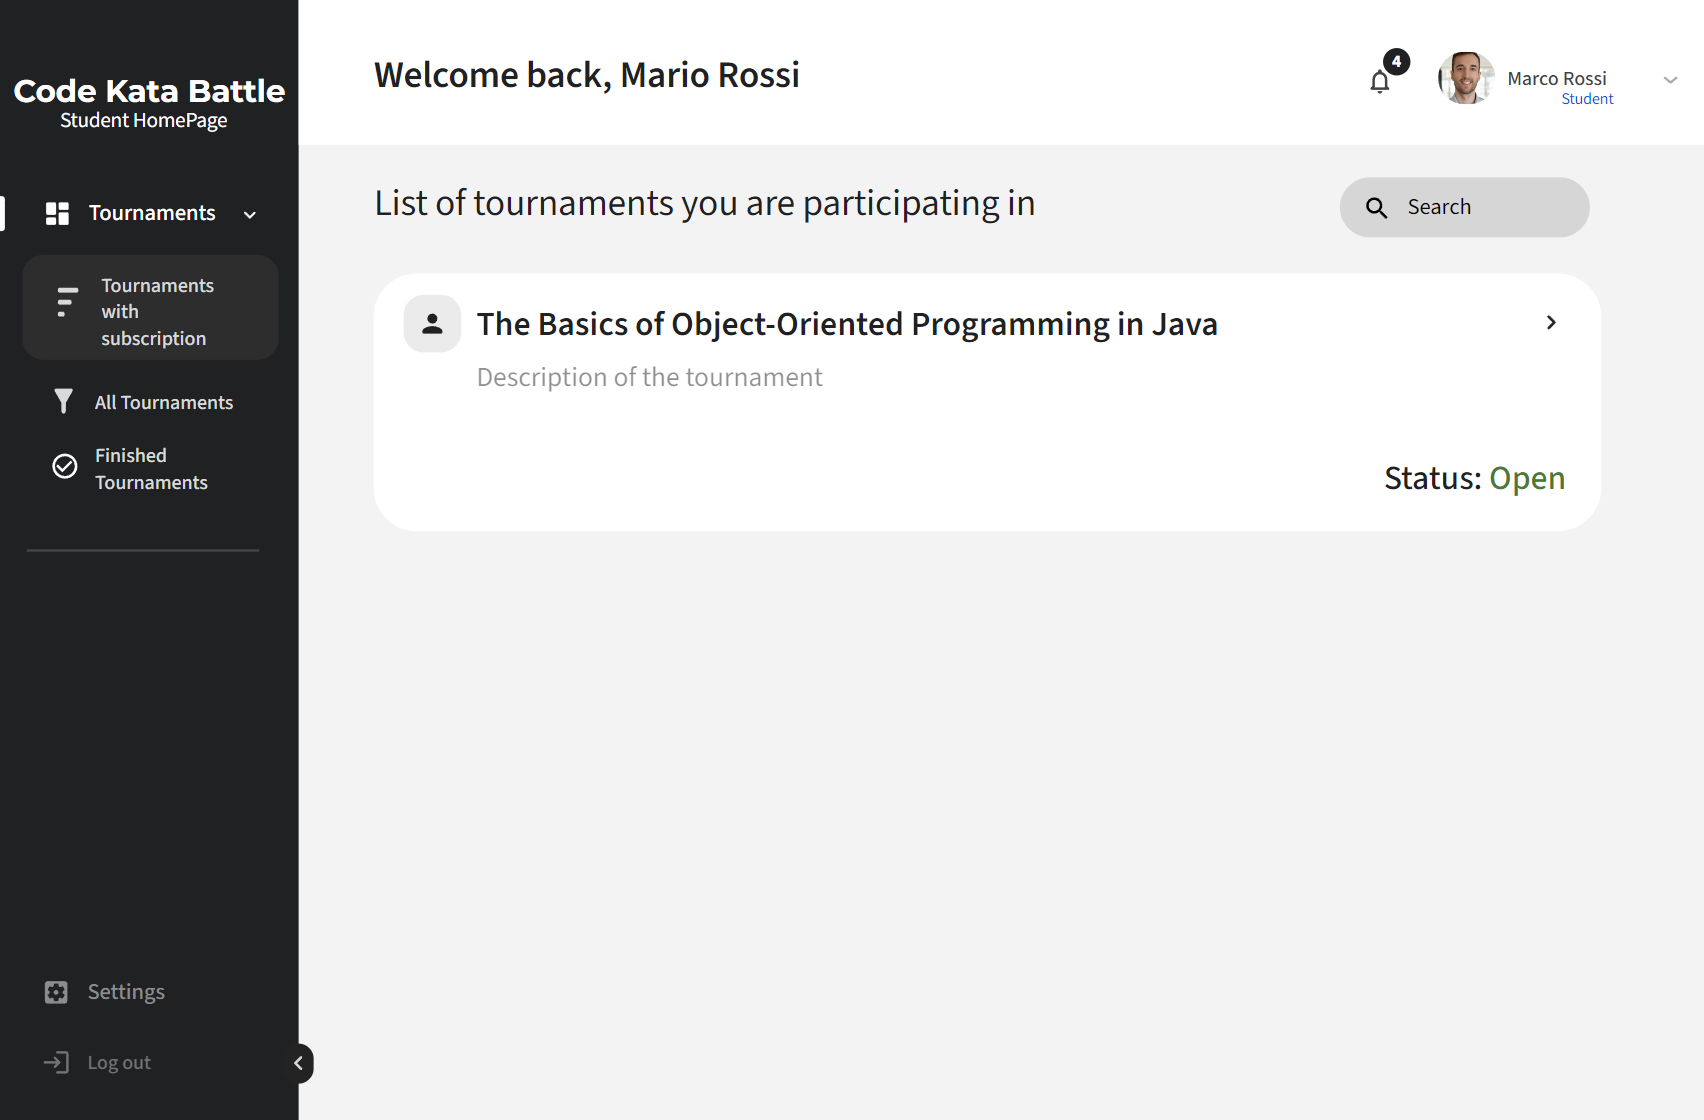
\includegraphics[width=\textwidth]{../images/homepage-student.png}
      \caption{HomePage Student}
      \label{fig:HomePage Student}
\end{figure}
\begin{figure}[H]
      \centering
      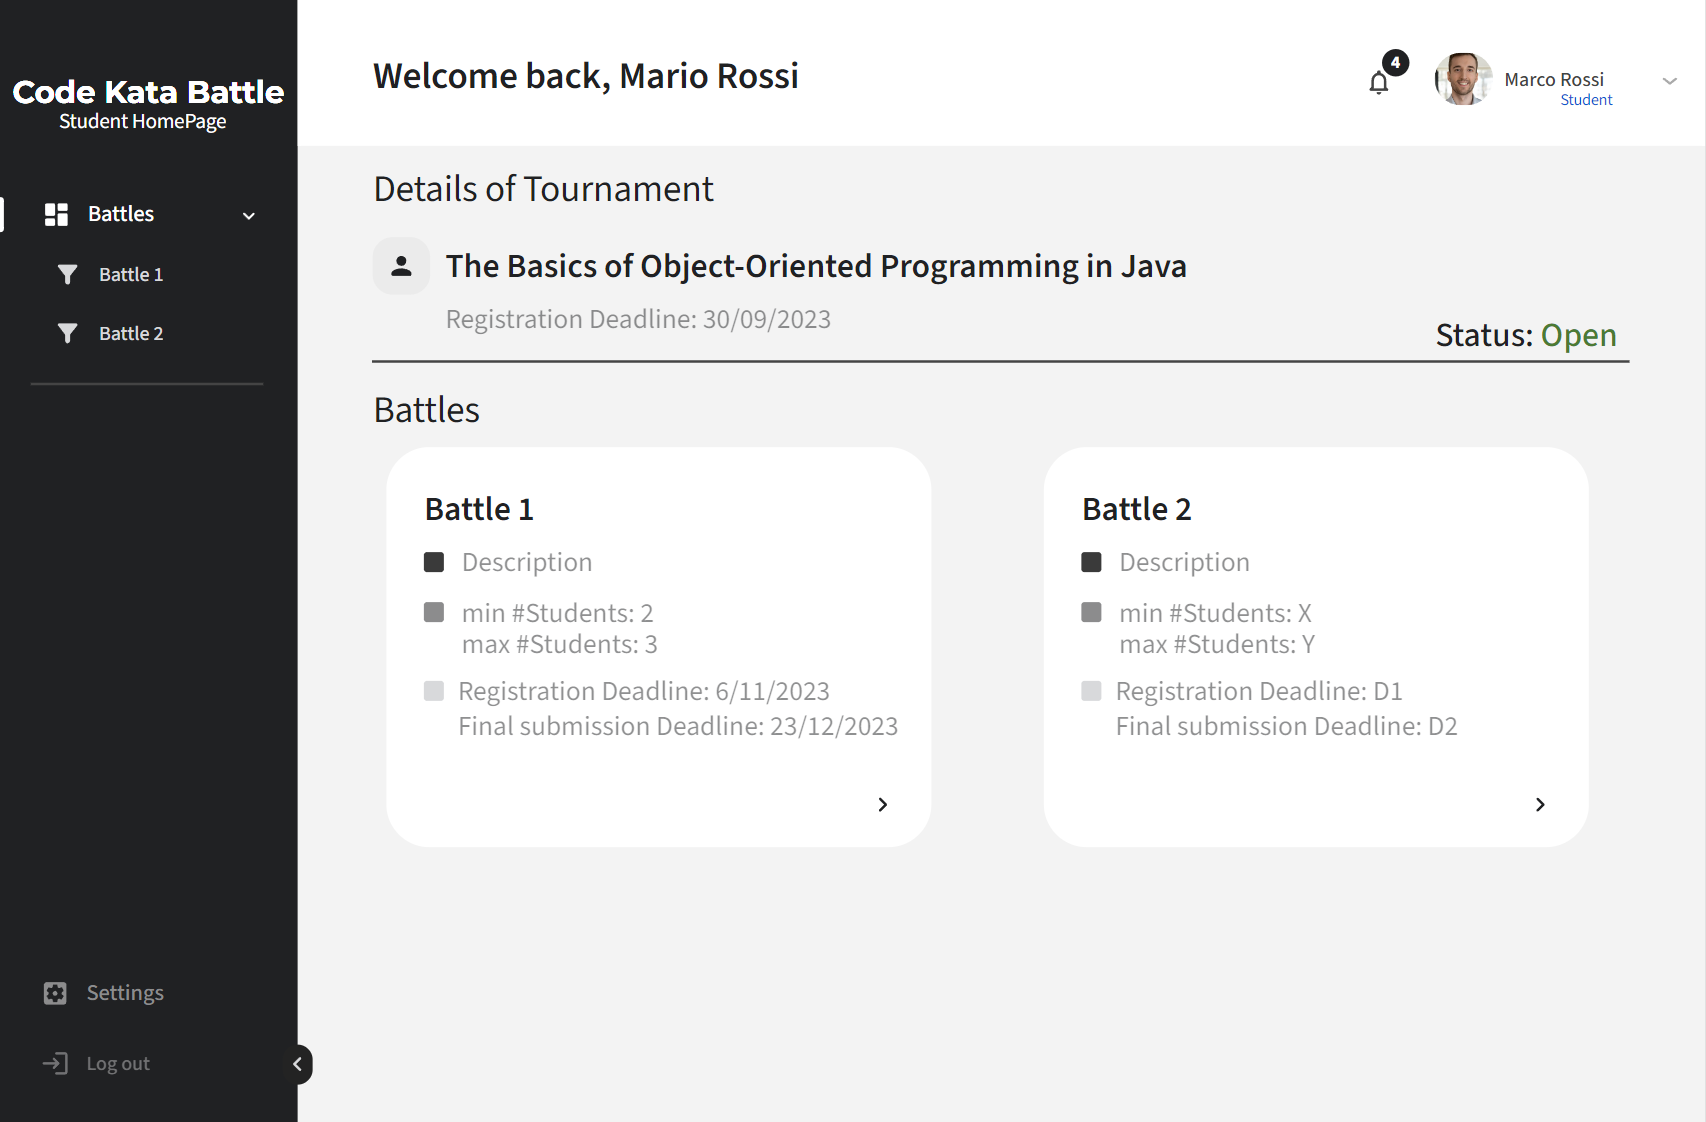
\includegraphics[width=\textwidth]{../images/details-tournament-student.png}
      \caption{Details Tournament Student}
      \label{fig:Details Tournament Student}
\end{figure}

\subsection{Hardware Interfaces}
The system does not need any specific hardware, each user will need a smartphone
or a computer with an Internet connection in order to communicate with the servers
of the platform.

\subsection{Software Interfaces}
The system will need to interface with the following software:
\begin{enumerate}
      \item \textbf{A git-compatible software~\cite{EmbeddingGit},~\cite{JGit}} {-} in order to create git repositories for
            the battles, push them to Github and clone students repositories in order to evaluate
            them
      \item \textbf{Language-specific software build systems} {-} in order to be able to build
            the students projects for evaluation. Different languages have their own
            requirements for compiling and executing code, so for each supported language
            the system will need to interact with one or more tools, at minimum with a
            compiler or interpreter (e.g gcc or clang for C/C++, javac for Java, node for
            JavaScript) but more likely with more complex tools (such as make for C/C++,
            Maven or Gradle for Java, npm for JavaScript)
      \item \textbf{Language-specific test suites} {-} in order to evaluate which
            tests have been passed or failed. Once again, each supported language
            will need their own implementation, at best by communicating directly
            with a testing framework (such as junit for Java or Jest for JavaScript)
            or a build tool (such as Gradle), at worst by directly parsing the text
            output of tests.
      \item \textbf{Static analysis tools} {-} in order to be used for scoring
            (\cite{WikipediaStaticAnalysis}, \cite{GhStaticAnalysis}). In this
            case, a choice can be made between interfacing with more lower-level software
            specific tools, which can potentially need per-language support (such as
            Errorprone, SpotBugs for Java or ESLint for Javascript), tools which already
            support a plethora of languages out of the box (such as Infer), or higher level
            platforms which already interface on their own the lower-level tools (such as
            SonarQube \cite{SonarQube})
      \item \textbf{A language interpreter} {-} to be used to declare variables and evaluate
            them to be used for the assignment of badges to students. A decision must be made
            between developing a custom language with its interpreter or the use of an already
            available interpreted language such as Javascript or Lua, with the consequent
            integration needed and the additional constraints to apply in order to disallow
            potential malicious use
\end{enumerate}
Additionally, in order to implement the gamification aspect, additional information
from each of these tools might be required in order to be able to define variables
for badges. For example, we might need to extract more metadata from git
related to number of commits by each student, lines changed, the dates of
the first/last commit, etc so that educators are able to use those.

\subsection{Communication Interfaces}
The system will need to communicate with the following external platforms:
\begin{enumerate}
      \item \textbf{GitHub} {-} which is used for code-hosting. The system will need to
            communicate with GitHub using the git protocol either over HTTP or SSH in order
            to manage and interact with repositories, but will also need to possibly interact
            with the GitHub API over HTTP (using their REST API \cite{GitHubRest}
            or their GraphQL API \cite{GitHubGraphQL}) to
            create new repositories, as well as to collect additional metadata to be used
            for gamification variables. Additionally, it will also need to receive messages
            from GitHub workflows, so an API will need to be exposed so that a workflow
            will be able to notify the system of the push of a new commit by a student
      \item \textbf{External static analysis platforms} {-} in case they are choosen to
            implement static analysis. For example if SonarQube is used, the system will
            need to be able to communicate using its API to receive reports about projects \cite{SonarQubeExt}
      \item \textbf{3rd party SSO API} {-} in order to integrate automatically with the
            universities, to avoid having to manually register each student over, we might
            need to communicate with their specific Sign On system
\end{enumerate}

Therefore, the following communication protocols are used:
\begin{enumerate}
      \item \textbf{HyperText Transfer Protocol over Secure Socket Layer (HTTPS)} {-} used
            for all external communications
      \item \textbf{Secure Shell (SSH)} {-} used for git communications. This is to be
            preferred to HTTPS as the use of SSH certificates will also need to more easily
            and securely authenticate the system to the GitHub platform \cite{GitHubSSH}
      \item \textbf{GraphQL~\cite{GraphQL}} {-} on top of HTTPS used for communicating with GitHub
\end{enumerate}

\section{Functional Requirements}

\begin{enumerate}[label=\textbf{R\arabic*}:,ref=R\arabic*,leftmargin=1.3cm]
      \labelleditem{The system shall allow users to login with SSO}
      \labelleditem{The system shall allow the educator to create a tournament.}
      \begin{enumerate}[label=\textbf{R\arabic{enumi}.\arabic*}:,ref=R\arabic{enumi}.\arabic*, leftmargin=*]
            \labelledsubitem{The system shall allow the educator to specify the subscribe deadline of a tournament.}
            \labelledsubitem{The system shall allow the educator to grant other colleagues the permission to create battles within the context of a specific tournament.}
            \labelledsubitem{The system shall notify the students of the new tournament.}
            \labelledsubitem{The system shall allow the educator who create the tournament to close it.}
      \end{enumerate}
      \labelleditem{The system shall allow students to subscribe to a tournament.}
      \labelleditem{The system shall allow the educator to create a battle within the context of a specific tournament.}
      \begin{enumerate}[label=\textbf{R\arabic{enumi}.\arabic*}:,ref=R\arabic{enumi}.\arabic*, leftmargin=*]
            \labelledsubitem{The system shall allow the educator to set minimum and maximum number of students per group.}
            \labelledsubitem{The system shall allow the educator to set a textual description.}
            \labelledsubitem{The system shall allow the educator to set the programming language.}
            \labelledsubitem{The system shall allow the educator to upload a set of test cases.}
            \labelledsubitem{The system shall allow the educator to upload a build automation script.}
            \labelledsubitem{The system shall allow the educator to set a registration deadline.}
            \labelledsubitem{The system shall allow the educator to set a final submission deadline.}
            \labelledsubitem{The system shall allow the educator to enable manual evaluation.}
            \labelledsubitem{The system shall allow the educator to select aspects that should be evaluated by the static analysis tool, such as security, reliability, and maintainability.}
            \labelledsubitem{The system shall notify students subscribed to a tournament of the creation of a new battle.}
      \end{enumerate}
      \labelleditem{The system shall allow students to join a battle, respecting the minimum and maximum number of students per group.}
      \begin{enumerate}[label=\textbf{R\arabic{enumi}.\arabic*}:,ref=R\arabic{enumi}.\arabic*, leftmargin=*]
            \labelledsubitem{The system shall allow students to invite other students to join a battle.}
            \labelledsubitem{The system shall allow students to accept received invitation.}
      \end{enumerate}
      \labelleditem{When the registration deadline expires, the system shall create a GitHub repository containing the code kata.}
      \labelleditem{The system shall send the link to all students who are members of subscribed teams.}
      \labelleditem{The system shall expose an API that can by called by the GitHub Action platform.}
      \labelleditem{On each push, the system shall calculate and update the battle score of the team.}
      \begin{enumerate}[label=\textbf{R\arabic{enumi}.\arabic*}:,ref=R\arabic{enumi}.\arabic*, leftmargin=*]
            \labelledsubitem{The system shall pull the latest sources.}
            \labelledsubitem{The system shall analyze quality level of the sources, based on the aspect selected by the educator.}
            \labelledsubitem{The system shall run tests uploaded by the educator.}
            \labelledsubitem{The system shall measure the time passed between the registration deadline and the last commit.}
      \end{enumerate}
      \labelleditem{The system shall allow students and educators involved in the battle to see the current rank evolving during the battle.}
      \labelleditem{When the submission deadline expires, if manual evaluation is required, the system shall change the state of the battle to the consolidation stage.}
      \labelleditem{When the submission deadline expires, if manual evaluation is not required, the system shall close the battle.}
      \labelleditem{During the consolidation stage, if manual evaluation is required, the system shall allow the educator to go through the sources produced by each team to assign his/her score.}
      \labelleditem{At the end of a battle, the system shall calculate the final rank.}
      \labelleditem{When the final rank is available, the system shall notify all students participating in the battle.}
      \labelleditem{At the end of each battle, the platform updates the personal tournament score of each student, that is the sum of all battle scores received in that tournament.}
      \labelleditem{The system shall allows users to see the tournament ranks.}
      \labelleditem{At the end of a tournament, the system shall calculate the final tournament rank.}
      \labelleditem{When the final tournament rank is available, the system shall notify all students involved in the tournament.}
      \labelleditem{The system shall allow the educator who create a tournament, to create badges within the context of the tournament.}
      \begin{enumerate}[label=\textbf{R\arabic{enumi}.\arabic*}:,ref=R\arabic{enumi}.\arabic*, leftmargin=*]
            \labelledsubitem{The system shall allow the educator to specify the title of the badge.}
            \labelledsubitem{The system shall allow the educator to create a new variable that represent any piece of information available in the platform relevant for scoring.}
            \labelledsubitem{The system shall allow the educator to specify one or more rules that must be fulfilled to achieve the badge, based on variables.}
            \labelledsubitem{The system shall allow users to visualize badges collected by a student.}
      \end{enumerate}
      \labelleditem{At the end of a tournament, the system shall assign badges to the student who fulfilled the rules.}
\end{enumerate}

\pagebreak

\subsection{Use case diagrams}
\subsubsection{Student}

\begin{figure}[H]
      \centering
      \puml{puml/UC-diagram-student}
      \caption{Student use case diagram}
      \label{fig:Student use case diagram}
\end{figure}

\subsubsection{Educator}
\begin{figure}[H]
      \centering
      \puml{puml/UC-diagram-educator}
      \caption{Educator use case diagram}
      \label{fig:Educator use case diagram}
\end{figure}

\pagebreak

\subsection{Use cases}
%Oppure facciamo tre sezioni separate per tabella, seq diagram e activity diagram,
% ma così mi sembra più leggibile.
\begin{enumerate}[label=\textbf{UC\arabic*}:,ref=UC\arabic*,leftmargin=1.3cm]
      \newcounter{resumeEnumeration}

      \labelleditem{
            \textbf{}
            \begin{table}[H]
                  %\caption*{\textbf{Title}}
                  \centering
                  \begin{tabular}{|l|p{11.9cm}|}
                        \hline
                        \textbf{Name}            & Educator creates a new Tournament                                                                 \\\hline
                        \textbf{Actor}           & Educator who wants to create the tournament, Students                                             \\\hline
                        \textbf{Entry condition} &
                        \begin{itemize}
                              \item Educator is logged in
                        \end{itemize}                                                                                                   \\\hline
                        \textbf{Event flow}      &
                        \begin{enumerate}[label=\arabic*.]
                              \item The educator selects the option to create a new tournament
                              \item The educator inserts the name of the tournament.
                              \item The educator inserts the registration deadline of the tournament.
                              \item The educator selects all the other educators he wants to invite to allow them to create new battles for the tournament.
                              \item The educator \hyperref[{{UC2}}]{creates a set of badges}.
                              \item The educator confirms the creation of the tournament.
                              \item The platform creates the new tournament.
                              \item The platform sends to the educator a confirmation message.
                              \item The platform sends a notification to all students in the platform.
                        \end{enumerate} \\\hline
                        \textbf{Exit condition}  & The new tournament is created                                                                     \\\hline
                        \textbf{Exception}       & The name of the tournament already exists.
                        In that case, the platform returns an error and does not create the tournament.                                              \\\hline
                  \end{tabular}
                  \caption{Educator creates a new Tournament }
                  \label{table:Educator creates a new Tournament }
            \end{table}
            \begin{adjustbox}{
                        max size={\textwidth}{\textheightwithcaption{1}},
                        caption={Educator creates a new Tournament},
                        label={fig:Educator creates a new Tournament},
                        figure=H}
                  \centering
                  \puml{puml/UC1}
            \end{adjustbox}
            \pagebreak
      }
      \labelleditem{
            \textbf{}
            \begin{table}[H]
                  %\caption*{\textbf{Title}}
                  \centering
                  \begin{tabular}{|l|p{11.9cm}|}
                        \hline
                        \textbf{Name}            & Educator creates a new badge                        \\\hline
                        \textbf{Actor}           & Educator who wants to create badges                 \\\hline
                        \textbf{Entry condition} &
                        \begin{itemize}
                              \item Educator is logged in
                              \item Educator is creating a tournament
                        \end{itemize}                                         \\\hline
                        \textbf{Event flow}      &
                        \begin{enumerate}[label=\arabic*.]
                              \item The educator selects the option to create a new badge
                              \item The educator inserts the title of the badge.
                              \item The educator write Javascript code to create new variables.
                              \item The educator write one or more rules.
                              \item The educator click the confirmation button.
                              \item The platform create the new badge in the current tournament.
                              \item The platform shows a confirmation massage.
                        \end{enumerate}              \\\hline
                        \textbf{Exit condition}  & The new badges is created in the current tournament \\\hline
                        \textbf{Exception}       & The rules contains undefined variables.
                        In that case, the platform returns an error and does not create the badge.     \\\hline
                  \end{tabular}
                  \caption{Educator creates a new badge }
                  \label{table:Educator creates a new badge }
            \end{table}
            \begin{adjustbox}{
                        max size={\textwidth}{\textheightwithcaption{1}},
                        caption={Educator creates a new badge},
                        label={fig:Educator creates a new badge},
                        figure=H}
                  \centering
                  \puml{puml/UC2}
            \end{adjustbox}
            \pagebreak
      }
      \labelleditem{
            \textbf{}
            \begin{table}[H]
                  %\caption*{\textbf{Title}}
                  \centering
                  \begin{tabular}{|l|p{11.9cm}|}
                        \hline
                        \textbf{Name}            & Educator creates a new Battle for an Existing Tournament                                                                                                    \\\hline
                        \textbf{Actor}           & Educator who wants to create the battle, Students partecipating in the tournament                                                                           \\\hline
                        \textbf{Entry condition} &
                        \begin{itemize}
                              \item Educator is logged in
                              \item Educator has permission to modify the tournament
                        \end{itemize}                                                                                                                                  \\\hline
                        \textbf{Event flow}      &
                        \begin{enumerate}[label=\arabic*.]
                              \item The educator asks the platform the list of available tournaments.
                              \item The platform sends to the educator the list of available tournaments.
                              \item The educator selects the tournament.
                              \item The platform shows the detail of the selected tournament.
                              \item The educator inserts the Battle Description field.
                              \item The educator uploads test cases and build and automation scripts.
                              \item The educator inserts the minimum and maximum number of students per group.
                              \item The educator inserts the registration deadline.
                              \item The educator inserts the final submission deadline.
                              \item The educator selects the option to create the new battle.
                              \item The platform creates the battle for the tournament.
                              \item The platform sends to the educator a confirmation message.
                              \item The platform sends a notification to all students partecipating in the tournament.
                        \end{enumerate}                                                                                                \\\hline
                        \textbf{Exit condition}  & The new battle is added to the tournament                                                                                                                   \\\hline
                        \textbf{Exception}       & Some parameters are unfeasible (such as final submission deadline succeed the registration deadline, min number of students > max number of students, ...).
                        In that case, the platform returns an error and does not create the battle.                                                                                                            \\\hline
                  \end{tabular}
                  \caption{Educator creates a new Battle for an Existing Tournament        }
                  \label{table:Educator creates a new Battle for an Existing Tournament         }
            \end{table}
            \pagebreak
            \begin{adjustbox}{
                        max size={\textwidth}{\textheightwithcaption{1}},
                        caption={Educator creates a new Battle for an Existing Tournament},
                        label={fig:Educator creates a new Battle for an Existing Tournament},
                        figure=H}
                  \centering
                  \puml{puml/UC3}
            \end{adjustbox}
            \pagebreak
      }
      \labelleditem{
            \textbf{}
            \begin{table}[H]
                  %\caption*{\textbf{Title}}
                  \centering
                  \begin{tabular}{|l|p{11.9cm}|}
                        \hline
                        \textbf{Name}            & Student joins to an existing Tournament by receiving a notification                                     \\\hline
                        \textbf{Actor}           & Student                                                                                                 \\\hline
                        \textbf{Entry condition} &
                        \begin{itemize}
                              \item Student is logged in
                              \item A new tournament has been created
                              \item Student has received a notification of the creation of a new tournament
                        \end{itemize}                                                       \\\hline
                        \textbf{Event flow}      &
                        \begin{enumerate}[label=\arabic*.]
                              \item Upon the creation of a new tournament, the platform sends a notification to all students which have enabled them
                              \item The student asks the platform the list of available tournaments.
                              \item The platform sends to the student the list of available tournaments.
                              \item The student selects the tournament.
                              \item The platform sends to the student the detail of the selected tournament.
                              \item The student selects the option to sign up to the tournament.
                              \item The platform enrolls the student in the tournament.
                              \item The platform sends to the student a confirmation message.
                        \end{enumerate}              \\\hline
                        \textbf{Exit condition}  & The student is subscribed to the tournament                                                             \\\hline
                        \textbf{Exception}       & The student selects the option to sign up to the tournament when the registration deadline has expired.
                        In that case, the platform returns an error.                                                                                       \\\hline
                  \end{tabular}
                  \caption{Student joins to an existing Tournament by receiving a notication}
                  \label{table:Student joins to an existing Tournament by receiving a notication}
            \end{table}
            \begin{adjustbox}{
                        max size={\textwidth}{\textheightwithcaption{1}},
                        caption={Student joins to an existing Tournament by receiving a notication},
                        label={fig:Student joins to an existing Tournament by receiving a notication},
                        figure=H}
                  \centering
                  \puml{puml/UC4}
            \end{adjustbox}
            \pagebreak
      }
      \labelleditem{
            \textbf{}
            \begin{longtable}{|l|p{11.9cm}|}
                  \caption{Students create a team for a tournament battle}
                  \label{table:Students create a team for a tournament battle}
                  \endlastfoot
                  \hline
                  \textbf{Name}            & Students create a team for a tournament battle                                                                            \\\hline
                  \textbf{Actor}           & Inviting student, Invited student 1, Invited student 2                                                                    \\\hline
                  \textbf{Entry condition} &
                  \begin{itemize}
                        \item Students are logged in
                        \item Students are enrolled in the same tournament
                        \item Students has invitation notifications enabled
                  \end{itemize}                                                                                                   \\\hline
                  \textbf{Event flow}      &
                  \begin{enumerate}[label=\arabic*.]
                        \item The inviting student asks the platform the list of available tournaments.
                        \item The platform sends to the inviting student the list of available tournaments.
                        \item The inviting student selects the tournament.
                        \item The platform sends to the inviting student the detail of the selected tournament (including the battles available for the tournament).
                        \item The inviting student selects the battle in the tournament.
                        \item The platform sends to the inviting student the detail of the selected battle within the tournament.
                        \item The inviting student selects the option to create a new team for the battle.
                        \item The platform creates a new team for the battle.
                        \item The platform add the inviting student to the created team.
                        \item The platform returns to the inviting student a confirmation message.
                        \item The inviting student selects the option to invite "invited student 1".
                        \item The platform creates an invitation for invited student 1.
                        \item The platform sends a notification to invited student 1.
                        \item Invited student 1 receives the notification and accepts.
                        \item The platform adds invited student 1 to the team.
                        \item The platform returns to invited student 1 a confirmation message.
                        \item The inviting student selects the option to invite "invited student 2".
                        \item The platform creates an invitation for invited student 2.
                        \item Invited student 2 asks the platform the list of invites.
                              \setcounter{resumeEnumeration}{\value{enumii}}
                              % Manually split the cell cause longtable cannot do it
                  \end{enumerate}          \\\hline
                                           &
                  \begin{enumerate}[label=\arabic*.]
                        \setcounter{enumii}{\value{resumeEnumeration}}
                        \item The platform returns to Invited student 2 the list of his invites.
                        \item Invited student 2 accepts the invite for the battle.
                        \item The platform adds invited student 2 to the team.
                        \item The platform returns to invited student 2 a confirmation message.
                        \item The inviting student selects the option to partecipate in the battle with the new created team.
                        \item The platform signs up the team to the battle.
                        \item The platform returns to inviting student a confirmation message.
                  \end{enumerate}                                                 \\\hline
                  \textbf{Exit condition}  & The students are all subscribed in a battle with the same team                                                            \\\hline
                  \textbf{Exception}       & \begin{itemize}
                                                   \item Inviting student wants to invite another student but the maximum number of students has been reached.
                                                         In that case, the platform returns an error.
                                                   \item The team wants to participate in a battle but the number of participants requirement of the battle is not satisfied.
                                                         In that case, the platform returns an error and the student can invite additional members.
                                             \end{itemize} \\\hline
            \end{longtable}
            \pagebreak
            \begin{adjustbox}{
                        max size={\textwidth}{\textheightwithcaption{1}},
                        caption={Students create a team for a tournament battle},
                        label={fig:Students create a team for a tournament battle},
                        figure=H}
                  \centering
                  \puml{puml/UC5}
            \end{adjustbox}
            \pagebreak
      }
      \labelleditem{
            \textbf{}
            \begin{table}[H]
                  %\caption*{\textbf{Title}}
                  \centering
                  \begin{tabular}{|l|p{11.9cm}|}
                        \hline
                        \textbf{Name}            & Student forks the repository                                                                                      \\\hline
                        \textbf{Actor}           & Forking student, teammates, GitHub                                                                                \\\hline
                        \textbf{Entry condition} &
                        \begin{itemize}
                              \item Students have created a team
                              \item The team is subscribed to a battle
                        \end{itemize}                                                                                                      \\\hline
                        \textbf{Event flow}      &
                        \begin{enumerate}[label=\arabic*.]
                              \item When the registration deadline of a battle expires, the platform creates the repository GitHub with name and description of the battle.
                              \item The platform uploads to the repository the build automation scripts and public tests
                              \item The platform notifies all students subscribed to the battle.
                              \item The student fork the repository.
                              \item The student adds his teammates as collaborators in the repository.
                              \item The student enables GitHub Action.
                              \item The student insert in the platform the link to his repository.
                        \end{enumerate} \\\hline
                        \textbf{Exit condition}  & The GitHub repository for the battle is created                                                                   \\\hline
                        %\textbf{Exception} &                                                                                              \\\hline
                  \end{tabular}
                  \caption{Student forks the repository}
                  \label{table:Student forks the repository}
            \end{table}
            \begin{adjustbox}{
                        max size={\textwidth}{\textheightwithcaption{1}},
                        caption={Student forks the repository},
                        label={fig:Student forks the repository},
                        figure=H}
                  \centering
                  \puml{puml/UC6}
            \end{adjustbox}
            \pagebreak
      }
      \labelleditem{
            \textbf{}
            \begin{table}[H]
                  %\caption*{\textbf{Title}}
                  \centering
                  \begin{tabular}{|l|p{11.9cm}|}
                        \hline
                        \textbf{Name}            & Students pushes and triggers automatic evaluation                                                                 \\\hline
                        \textbf{Actor}           & Pushing Student, Students participating in the same team, GitHub, Static analysis tool                            \\\hline
                        \textbf{Entry condition} &
                        \begin{itemize}
                              \item Pushing Student is participating in a battle of a tournament
                              \item Pushing Student has forked the GitHub repository of the battle
                              \item Pushing Student has set up the GitHub action on the forked repository
                              \item Pushing Student has inserted the repository link in the platform
                        \end{itemize}                                                                   \\\hline
                        \textbf{Event flow}      &
                        \begin{enumerate}[label=\arabic*.]
                              \item The pushing Student commits project code.
                              \item The pushing Student pushes the committed project code to the forked GitHub battle repository.
                              \item The GitHub Action platform notifies the CKB platform about the new push.
                              \item The platform pulls the updated project code.
                              \item The platform builds the project.
                              \item The platform runs all the test cases (public and private) associated with the battle.
                              \item The platform calculates the days that have passed since the start of the battle.
                              \item The platform runs the static analysis tool.
                              \item The platform calculates the total score.
                              \item The platform updates the battle team score.
                              \item The platform notifies the updated battle team score to all the students of the same team.
                        \end{enumerate}                                           \\\hline
                        \textbf{Exit condition}  & The battle team score is updated                                                                                  \\\hline
                        \textbf{Exception}       & The platform receives a push notification from an unauthorized repository. In this case the request is discarded. \\\hline
                        \textbf{Special reqs}    & The platform must evaluate the project within 10 minutes of the push.                                             \\\hline
                  \end{tabular}
                  \caption{Students pushes and triggers automatic evaluation}
                  \label{table:Students pushes and triggers automatic evaluation}
            \end{table}
            \begin{adjustbox}{
                        max size={\textwidth}{\textheightwithcaption{2}},
                        caption={Students pushes and triggers automatic evaluation},
                        label={fig:Students pushes and triggers automatic evaluation},
                        figure=H}
                  \centering
                  \puml{puml/UC7}
            \end{adjustbox}
            \pagebreak
      }
      \labelleditem{
            \textbf{}
            \begin{table}[H]
                  %\caption*{\textbf{Title}}
                  \centering
                  \begin{tabular}{|l|p{11.9cm}|}
                        \hline
                        \textbf{Name}            & Educator manually evaluates teams                                                                          \\\hline
                        \textbf{Actor}           & Educator, Students, GitHub                                                                                 \\\hline
                        \textbf{Entry condition} &
                        \begin{itemize}
                              \item Educator has logged in
                              \item Educator has permission to modify the battle of the tournament
                        \end{itemize}                                                                   \\\hline
                        \textbf{Event flow}      &
                        \begin{enumerate}[label=\arabic*.]
                              \item When the submission deadline expires, the platform opens the consolidation stage.
                              \item The educator asks the platform the the list of available tournaments.
                              \item The platform sends to the educator the list of available tournaments.
                              \item The educator selects the tournament.
                              \item The platform shows the detail of the selected tournament (including the list of battles).
                              \item The educator selects the battle.
                              \item The platform shows the details of the battle.
                              \item The educator selects the option to evaluate teams.
                              \item The platform returns the list of teams within the battle.
                              \item The educator asks for the source code for each team.
                              \item The platform returns to the educator the source code for each team.
                              \item The educator assigns a score to each team.
                              \item The educator selects the option to close the battle.
                              \item The platform calculates the final battle ranks.
                              \item The platform updates the personal tournament score of each student.
                              \item The platform notifies students who participated in the battle.
                              \item The platform sends to the educator a confirmation message.
                        \end{enumerate}                                        \\\hline
                        \textbf{Exit condition}  & The battle is closed, the final battle ranks are calculated and the personal tournament scores are updated \\\hline
                        \textbf{Exception}       & The educator selects the option to close the battle before evaluating all students.
                        In this case the platform return an error and the educator can assign the missing grades.                                             \\\hline
                        %\textbf{Special reqs}    &                                                      \\\hline
                  \end{tabular}
                  \caption{Educator manually evaluate teams    }
                  \label{table:Educator manually evaluate teams    }
            \end{table}
            \begin{adjustbox}{
                        max size={\textwidth}{\textheightwithcaption{1}},
                        caption={Educator manually evaluate teams},
                        label={fig:Educator manually evaluate teams},
                        figure=H}
                  \centering
                  \puml{puml/UC8}
            \end{adjustbox}
            \pagebreak
      }
      \labelleditem{
            \textbf{}
            \begin{table}[H]
                  %\caption*{\textbf{Title}}
                  \centering
                  \begin{tabular}{|l|p{11.9cm}|}
                        \hline
                        \textbf{Name}            & Educator closes a tournament                               \\\hline
                        \textbf{Actor}           & Educator, Students                                         \\\hline
                        \textbf{Entry condition} &
                        \begin{itemize}
                              \item Educator has logged in
                              \item Educator has permission to modify the tournament
                              \item All battles in the tournament are closed
                        \end{itemize}                                 \\\hline
                        \textbf{Event flow}      &
                        \begin{enumerate}[label=\arabic*.]
                              \item The educator asks the platform the list of available tournaments.
                              \item The platform sends to the educator the list of available tournaments.
                              \item The educator selects the tournament.
                              \item The platform shows the detail of the selected tournament.
                              \item Educator selects the option to close the tournament.
                              \item The platform calculates the final tournament rank.
                              \item The platform gets the information about the available badges for the tournament.
                              \item The platform assigns badges to the student who fulfilled the rules.
                              \item The platform notifies students who participated in the tournament.
                        \end{enumerate} \\\hline
                        \textbf{Exit condition}  & The tournament is closed and the badges are assigned       \\\hline
                        %\textbf{Exception}       &                                                      \\\hline
                        %\textbf{Special reqs}    &                                                      \\\hline
                  \end{tabular}
                  \caption{Educator closes a tournament   }
                  \label{table:Educator closes a tournament   }
            \end{table}
            \begin{adjustbox}{
                        max size={\textwidth}{\textheightwithcaption{1}},
                        caption={Educator closes a tournament},
                        label={fig:Educator closes a tournament},
                        figure=H}
                  \centering
                  \puml{puml/UC9}
            \end{adjustbox}
      }
\end{enumerate}
\pagebreak

\subsection{Requirements mapping}
In this section it is shown how the relation $R\land D \models G$ holds.
In particular, the following traceability matrix associates domain assumptions and requirements to goals.
After that, to facilitate reading, the text of all the assumptions and all the requirements related to each goal is reported.

\begin{table}[H]
      %\caption*{\textbf{Title}}
      \centering
      \begin{tabular}{|l|p{8cm}|p{5cm}|}
            \hline
            \textbf{Goal ID} & \textbf{Requirement ID}                                                                                                                                                                                                      & \textbf{Domain assumption ID}                                                                               \\\hline
            \ref{{G1}}       & \ref{{R1}}, \ref{{R2}}, \ref{{R2.1}}, \ref{{R2.4}}                                                                                                                                                                           & \ref{{D1}}, \ref{{D2}}, \ref{{D3}}, \ref{{D4}}                                                              \\\hline
            \ref{{G2}}       & \ref{{R1}}, \ref{{R4}}, \ref{{R4.1}}, \ref{{R4.2}}, \ref{{R4.3}}, \ref{{R4.4}}, \ref{{R4.5}}, \ref{{R4.6}}, \ref{{R4.7}}                                                                                                     & \ref{{D2}}, \ref{{D3}}, \ref{{D4}}                                                                          \\\hline
            \ref{{G3}}       & \ref{{R1}}, \ref{{R2.2}}                                                                                                                                                                                                     & \ref{{D2}}, \ref{{D3}}, \ref{{D4}}                                                                          \\\hline
            \ref{{G4}}       & \ref{{R1}}, \ref{{R4.8}}, \ref{{R4.9}}                                                                                                                                                                                       & \ref{{D2}}, \ref{{D3}}, \ref{{D4}}                                                                          \\\hline
            \ref{{G5}}       & \ref{{R1}}, \ref{{R2.3}}                                                                                                                                                                                                     & \ref{{D1}}, \ref{{D2}}, \ref{{D3}}, \ref{{D4}}                                                              \\\hline
            \ref{{G6}}       & \ref{{R1}}, \ref{{R3}}                                                                                                                                                                                                       & \ref{{D1}}, \ref{{D3}}, \ref{{D4}}                                                                          \\\hline
            \ref{{G7}}       & \ref{{R1}}, \ref{{R4.10}}                                                                                                                                                                                                    & \ref{{D1}}, \ref{{D3}}, \ref{{D4}}                                                                          \\\hline
            \ref{{G8}}       & \ref{{R1}}, \ref{{R5.1}}, \ref{{R5.2}}                                                                                                                                                                                       & \ref{{D1}}, \ref{{D3}}, \ref{{D4}}                                                                          \\\hline
            \ref{{G9}}       & \ref{{R1}}, \ref{{R5}}, \ref{{R6}}, \ref{{R7}}                                                                                                                                                                               & \ref{{D1}}, \ref{{D3}}, \ref{{D4}}, \ref{{D5}}                                                              \\\hline
            \ref{{G10}}      & \ref{{R1}}, \ref{{R8}}, \ref{{R9}}, \ref{{R9.1}}, \ref{{R9.2}}, \ref{{R9.3}}, \ref{{R9.4}}, \ref{{R10}}, \ref{{R11}}, \ref{{R12}}, \ref{{R13}}, \ref{{R14}}, \ref{{R15}}, \ref{{R16}}, \ref{{R17}}, \ref{{R18}}, \ref{{R19}} & \ref{{D1}}, \ref{{D3}}, \ref{{D4}}, \ref{{D5}}, \ref{{D6}}, \ref{{D7}}, \ref{{D8}}, \ref{{D9}}, \ref{{D10}} \\\hline
            \ref{{G11}}      & \ref{{R1}}, \ref{{R20}}, \ref{{R20.1}}, \ref{{R20.2}}, \ref{{R20.3}}                                                                                                                                                         & \ref{{D2}}, \ref{{D3}}, \ref{{D4}}                                                                          \\\hline
            \ref{{G12}}      & \ref{{R1}}, \ref{{R21}}                                                                                                                                                                                                      & \ref{{D1}}, \ref{{D3}}, \ref{{D4}}                                                                          \\\hline
            \ref{{G13}}      & \ref{{R1}}, \ref{{R20.4}}                                                                                                                                                                                                    & \ref{{D1}}, \ref{{D2}}, \ref{{D3}}, \ref{{D4}}                                                              \\\hline
      \end{tabular}
      \caption{Traceability matrix}
      \label{table:Traceability matrix}
\end{table}

\begin{enumerate}[leftmargin=1.3cm]
      \printitem{G1}
      \begin{enumerate}[leftmargin=1.3cm]
            \printitem{R1}
            \printitem{R2}
            \printitem{R2.1}
            \printitem{R2.4}
            \printitem{D1}
            \printitem{D2}
            \printitem{D3}
            \printitem{D4}
      \end{enumerate}

      \printitem{G2}
      \begin{enumerate}[leftmargin=1.3cm]
            \printitem{R1}
            \printitem{R4}
            \printitem{R4.1}
            \printitem{R4.2}
            \printitem{R4.3}
            \printitem{R4.4}
            \printitem{R4.5}
            \printitem{R4.6}
            \printitem{R4.7}
            \printitem{D2}
            \printitem{D3}
            \printitem{D4}
      \end{enumerate}
      \printitem{G3}
      \begin{enumerate}[leftmargin=1.3cm]
            \printitem{R1}
            \printitem{R2.2}
            \printitem{D2}
            \printitem{D3}
            \printitem{D4}
      \end{enumerate}
      \printitem{G4}
      \begin{enumerate}[leftmargin=1.3cm]
            \printitem{R1}
            \printitem{R4.8}
            \printitem{R4.9}
            \printitem{D2}
            \printitem{D3}
            \printitem{D4}
      \end{enumerate}
      \printitem{G5}
      \begin{enumerate}[leftmargin=1.3cm]
            \printitem{R1}
            \printitem{R2.3}
            \printitem{D1}
            \printitem{D2}
            \printitem{D3}
            \printitem{D4}
      \end{enumerate}
      \printitem{G6}
      \begin{enumerate}[leftmargin=1.3cm]
            \printitem{R1}
            \printitem{R3}
            \printitem{D1}
            \printitem{D3}
            \printitem{D4}
      \end{enumerate}
      \printitem{G7}
      \begin{enumerate}[leftmargin=1.3cm]
            \printitem{R1}
            \printitem{R4.10}
            \printitem{D1}
            \printitem{D3}
            \printitem{D4}
      \end{enumerate}
      \printitem{G8}
      \begin{enumerate}[leftmargin=1.3cm]
            \printitem{R1}
            \printitem{R5.1}
            \printitem{R5.2}
            \printitem{D1}
            \printitem{D3}
            \printitem{D4}
      \end{enumerate}
      \printitem{G9}
      \begin{enumerate}[leftmargin=1.3cm]
            \printitem{R1}
            \printitem{R5}
            \printitem{R6}
            \printitem{R7}
            \printitem{D1}
            \printitem{D3}
            \printitem{D4}
            \printitem{D5}
      \end{enumerate}
      \printitem{G10}
      \begin{enumerate}[leftmargin=1.3cm]
            \printitem{R1}
            \printitem{R8}
            \printitem{R9}
            \printitem{R9.1}
            \printitem{R9.2}
            \printitem{R9.3}
            \printitem{R9.4}
            \printitem{R10}
            \printitem{R11}
            \printitem{R12}
            \printitem{R13}
            \printitem{R14}
            \printitem{R15}
            \printitem{R16}
            \printitem{R17}
            \printitem{R18}
            \printitem{R19}
            \printitem{D1}
            \printitem{D3}
            \printitem{D4}
            \printitem{D5}
            \printitem{D6}
            \printitem{D7}
            \printitem{D8}
            \printitem{D9}
            \printitem{D10}
      \end{enumerate}
      \printitem{G11}
      \begin{enumerate}[leftmargin=1.3cm]
            \printitem{R1}
            \printitem{R20}
            \printitem{R20.1}
            \printitem{R20.2}
            \printitem{R20.3}
            \printitem{D2}
            \printitem{D3}
            \printitem{D4}
      \end{enumerate}
      \printitem{G12}
      \begin{enumerate}[leftmargin=1.3cm]
            \printitem{R1}
            \printitem{R21}
            \printitem{D1}
            \printitem{D3}
            \printitem{D4}
      \end{enumerate}
      \printitem{G13}
      \begin{enumerate}[leftmargin=1.3cm]
            \printitem{R1}
            \printitem{R20.4}
            \printitem{D1}
            \printitem{D2}
            \printitem{D3}
            \printitem{D4}
      \end{enumerate}
\end{enumerate}

The following traceability matrix associates requirements to use cases.
\begin{center}
      \begin{longtable}{|l|ccccccccc|}
            \hline
                                   & \textbf{\ref{{UC1}}} & \textbf{\ref{{UC2}}} & \textbf{\ref{{UC3}}} & \textbf{\ref{{UC4}}} & \textbf{\ref{{UC5}}} & \textbf{\ref{{UC6}}} & \textbf{\ref{{UC7}}} & \textbf{\ref{{UC8}}} & \textbf{\ref{{UC9}}} \\
            \hline
            \endhead
            \hline
            \endfoot
            \hline
            \caption{Use cases traceability matrix}
            \label{table:Use cases traceability matrix}
            \endlastfoot
            \textbf{\ref{{R1}}}    & \checkmark           & \checkmark           & \checkmark           & \checkmark           & \checkmark           & \checkmark           & \checkmark           & \checkmark           & \checkmark           \\
            \textbf{\ref{{R2}}}    & \checkmark           &                      &                      &                      &                      &                      &                      &                      &                      \\
            \textbf{\ref{{R2.1}}}  & \checkmark           &                      &                      &                      &                      &                      &                      &                      &                      \\
            \textbf{\ref{{R2.2}}}  & \checkmark           &                      &                      &                      &                      &                      &                      &                      &                      \\
            \textbf{\ref{{R2.3}}}  & \checkmark           &                      &                      & \checkmark           &                      &                      &                      &                      &                      \\
            \textbf{\ref{{R2.4}}}  &                      &                      &                      &                      &                      &                      &                      &                      & \checkmark           \\
            \textbf{\ref{{R3}}}    &                      &                      &                      & \checkmark           &                      &                      &                      &                      &                      \\
            \textbf{\ref{{R4}}}    &                      &                      & \checkmark           &                      &                      &                      &                      &                      &                      \\
            \textbf{\ref{{R4.1}}}  &                      &                      & \checkmark           &                      &                      &                      &                      &                      &                      \\
            \textbf{\ref{{R4.2}}}  &                      &                      & \checkmark           &                      &                      &                      &                      &                      &                      \\
            \textbf{\ref{{R4.3}}}  &                      &                      & \checkmark           &                      &                      &                      &                      &                      &                      \\
            \textbf{\ref{{R4.4}}}  &                      &                      & \checkmark           &                      &                      &                      &                      &                      &                      \\
            \textbf{\ref{{R4.5}}}  &                      &                      & \checkmark           &                      &                      &                      &                      &                      &                      \\
            \textbf{\ref{{R4.6}}}  &                      &                      & \checkmark           &                      &                      &                      &                      &                      &                      \\
            \textbf{\ref{{R4.7}}}  &                      &                      & \checkmark           &                      &                      &                      &                      &                      &                      \\
            \textbf{\ref{{R4.8}}}  &                      &                      & \checkmark           &                      &                      &                      &                      &                      &                      \\
            \textbf{\ref{{R4.9}}}  &                      &                      & \checkmark           &                      &                      &                      &                      &                      &                      \\
            \textbf{\ref{{R4.10}}} &                      &                      & \checkmark           &                      &                      &                      &                      &                      &                      \\
            \textbf{\ref{{R5}}}    &                      &                      &                      &                      & \checkmark           &                      &                      &                      &                      \\
            \textbf{\ref{{R5.1}}}  &                      &                      &                      &                      & \checkmark           &                      &                      &                      &                      \\
            \textbf{\ref{{R5.2}}}  &                      &                      &                      &                      & \checkmark           &                      &                      &                      &                      \\
            \textbf{\ref{{R6}}}    &                      &                      &                      &                      &                      & \checkmark           &                      &                      &                      \\
            \textbf{\ref{{R7}}}    &                      &                      &                      &                      &                      & \checkmark           &                      &                      &                      \\
            \textbf{\ref{{R8}}}    &                      &                      &                      &                      &                      &                      & \checkmark           &                      &                      \\
            \textbf{\ref{{R9}}}    &                      &                      &                      &                      &                      &                      & \checkmark           &                      &                      \\
            \textbf{\ref{{R9.1}}}  &                      &                      &                      &                      &                      &                      & \checkmark           &                      &                      \\
            \textbf{\ref{{R9.2}}}  &                      &                      &                      &                      &                      &                      & \checkmark           &                      &                      \\
            \textbf{\ref{{R9.3}}}  &                      &                      &                      &                      &                      &                      & \checkmark           &                      &                      \\
            \textbf{\ref{{R9.4}}}  &                      &                      &                      &                      &                      &                      & \checkmark           &                      &                      \\
            \textbf{\ref{{R10}}}   &                      &                      &                      &                      &                      &                      & \checkmark           &                      &                      \\
            \textbf{\ref{{R11}}}   &                      &                      &                      &                      &                      &                      &                      & \checkmark           &                      \\
            \textbf{\ref{{R12}}}   &                      &                      &                      &                      &                      &                      &                      & \checkmark           &                      \\
            \textbf{\ref{{R13}}}   &                      &                      &                      &                      &                      &                      &                      & \checkmark           &                      \\
            \textbf{\ref{{R14}}}   &                      &                      &                      &                      &                      &                      &                      & \checkmark           &                      \\
            \textbf{\ref{{R15}}}   &                      &                      &                      &                      &                      &                      &                      & \checkmark           &                      \\
            \textbf{\ref{{R16}}}   &                      &                      &                      &                      &                      &                      &                      & \checkmark           &                      \\
            \textbf{\ref{{R17}}}   &                      &                      &                      &                      &                      &                      &                      &                      & \checkmark           \\
            \textbf{\ref{{R18}}}   &                      &                      &                      &                      &                      &                      &                      &                      & \checkmark           \\
            \textbf{\ref{{R19}}}   &                      &                      &                      &                      &                      &                      &                      &                      & \checkmark           \\
            \textbf{\ref{{R20}}}   &                      & \checkmark           &                      &                      &                      &                      &                      &                      &                      \\
            \textbf{\ref{{R20.1}}} &                      & \checkmark           &                      &                      &                      &                      &                      &                      &                      \\
            \textbf{\ref{{R20.2}}} &                      & \checkmark           &                      &                      &                      &                      &                      &                      &                      \\
            \textbf{\ref{{R20.3}}} &                      & \checkmark           &                      &                      &                      &                      &                      &                      &                      \\
            \textbf{\ref{{R20.4}}} &                      &                      &                      &                      &                      &                      &                      &                      & \checkmark           \\
            \textbf{\ref{{R21}}}   &                      &                      &                      &                      &                      &                      &                      &                      & \checkmark           \\
      \end{longtable}
\end{center}

\pagebreak
\section{Performance Requirements}
The system must be sized considering the number of users who will use it.
Indeed, the grade assigned by the platform must not depend on the number of students pushing at the same time.

The automatic evaluation must be done within 10 minutes of the push.
If this does not happen, the platform can assume that the tests are deadlocked and kill the process.

The system must have disk space to store information of tournaments and battles, such as teams and ranks.
Students' code is hosted on GitHub, but it has to be cloned to the server disk to run tests.

\section{Design Constraints}
\subsection{Standards Compliance}
The CodeKataBattle (CKB) platform is designed with the goal of strictly adhering to several standards to ensure the quality, security and interoperability of the system.\\ The standards to which CKB adheres include:

\begin{enumerate}
      \item HTTPS Protocol Compliance\\
            Implementation of the HTTPS protocol according to the cryptographic standards established by IETF (Internet Engineering Task Force).

      \item Accessibility Standards\\
            Compliance with Web Content Accessibility Guidelines (WCAG) to ensure web accessibility.

      \item Security Standards\\
            Implementation of security best practices as defined by OWASP (Open Web Application Security Project) and NIST (National Institute of Standards and Technology).
            Such as password storage encryption with HASH512 + Salt, SSL Certificate and end-to-end communication encryption.


      \item API Interoperability\\
            Use of open standards for API design, such as RESTful API and adherence to specifications such as OpenAPI (Swagger).


      \item Coding Standards\\
            The platform follows universally accepted coding guidelines for the main programming language used in system development (e.g., Java or Python).
            Compliance with the coding guidelines for the main programming language (PEP 8 for Python, Java Coding Conventions for Java).


      \item Compliance with Privacy Regulations\\
            Compliance with privacy laws such as the General Data Protection Regulation (GDPR) for European citizens.
\end{enumerate}

\subsection{Hardware limitations}
Each student and educator must have an electronic device such as a computer or smartphone with an internet connection to
access the CKB Platform.
Students must be able to clone GitHub repositories on their device to participate in the various battles and accordingly must have a physical storage with sufficient space to store the sources and data of the various projects.
The device used must allow the student to view, edit, process and execute the sources.
The devices used by students and educators enable them to receive notifications.

\section{Software System Attributes}
\subsection{Reliability}
The CKB platform does not manage critical operations.
If an operation fails, it can be re-executed without any particular consequences.
For example, if the evaluation of an exercise fails, students can resubmit their code.
It is therefore reasonable to have a failure rate around 1\%.

\subsection{Availability}
The platform should have the lowest downtime possible during the day.
A few hours of downtime are allowed between 1am and 5am, when student are usually not studying.
The platform shall therefore guarantee 99\% (two-nines) of availability, so that 3.65 days of downtime per year are allowed.

\subsection{Security}
Communication between the user and the CBK platform is encrypted.
Furthermore, users must only be able to perform operations that they are authorized to do.
For example, a student must not be able to change his grade.

The CKB platform can be triggered through its API only from authorized repositories.

\subsection{Maintainability}
The system should be divided in scalable and reusable modules,
which will be easier to maintain and replace in case of failure.
Ordinary maintenance, for bug fixes and improvements, will be scheduled during night time, when the user traffic is minimal.

\subsection{Portability}
The CKD platform does not require any particular hardware or software.
It must be accessible from any operating system with a modern web browser.
A mobile application that allows users to see the state of the battles can also be developed.
Since the mobile app does not require any special function, a non-native approach can be adopted.
It is therefore possible to use cross-platform development tools, which can speed up the development process.